\lecture{11}{10.28}
\subsection{遗传算法}%
\label{sub:遗传算法}
\begin{notation}
    如何模拟物种繁殖:

    1. 种群中选择两个个体

    2. 随机确定编码序列断裂点

    3. 交换编码片段

    基因发生突变的概率称为遗传算法的\textbf{突变算子}
\end{notation}
\begin{notation}
    如何模拟竞争与选择:\textbf{适应度}
\end{notation}
\begin{eg}
    求函数$f\left( x \right) =x^2$ 的最大值,$x\in [0,31],x\in \mathbb{Z}$

    使用5个二进制码表示取值:$0\sim 31\Rightarrow \text{0b00000} \sim \text{0b11111}$ 

    定义32条染色体:
     \begin{table}[htpb]
        \centering
        \caption{染色体}
        \label{tab:染色体}
        \begin{tabular}{|c|c|}
        \hline
        $X_o$ & $X_b$ \\
        \hline
        0 & 0b00000\\
        1 & 0b00001\\
        $\ldots $ & $\ldots $ \\
        31 & 0b11111\\
        \hline
        \end{tabular}
    \end{table}
    
    假设初始种群数量$N=4$ ,随机产生20位的二进制串,每5个一组,得到4个初始个体

    如:0b\textbf{00110}10010\textbf{10011}01010

    适应度函数为给定问题$f\left( x \right) =x^2$
    \begin{table}[htpb]
        \centering
        \caption{选择算子}
        \label{tab:选择算子}
        \begin{tabular}{|c|c|c|c|c|c|c|}
        \hline
        编号 & 个体编码 & 个体 & 适应度 & $\displaystyle{\frac{f}{\sum f}} $ & $\displaystyle{\frac{4f}{\sum f}} $ & 生存数 \\
        \hline
        $S_1$ & 00110 & 6 & 36 & 0.043 & 0.175 & 0\\
        $S_2$ & 10010 & 18 & 324 & 0.394 & 1.578 & 2\\
        $S_3$ & 10011 & 19 & 361 & 0.439 & 1.759 & 2\\
        $S_4$ & 01010 & 10 & 100 & 0.121 & 0.487 & 0\\
        \hline
        \multicolumn{3}{|c|}{适应度总和} & 821 & \multicolumn{2}{|c|}{平均适应度} & 205.25\\
        \hline
        \end{tabular}
    \end{table}

    得到第一代种群:(0b10010, 0b10011), (0b10010, 0b10011):避免近亲相交

    令交叉概率$P_s=1$ ,变异概率$P_m=0.01$ (每五代变异一个基因),通过生存数生成新的种群,配对后随机选择断裂点位交叉配对,完成第一代遗传:第二代种群的适应度更高
    \begin{table}[htpb]
        \centering
        \caption{第一次交叉}
        \label{tab:第一次交叉}
        \begin{tabular}{|c|c|c|c|c|}
        \hline
        交叉前 & 交叉后 & 个体 & 适应度 & 生存数 \\
        \hline
        0b100\textbf{10} & 0b10011 & 19 & 361 & 1 \\
        0b100\textbf{11} & 0b10010 & 18 & 324 & 1 \\
        \hline
        0b1\textbf{0010} & 0b10011 & 19 & 361 & 1 \\
        0b1\textbf{0011} & 0b10010 & 18 & 324 & 1 \\
        \hline
        \multicolumn{3}{|c|}{适应度总和} & \multicolumn{2}{|c|}{821 $\Rightarrow $ 1370}\\
        \hline
        \end{tabular}
    \end{table}

    生成第五代种群后,通过变异算子随机挑选一个基因进行改变

    经过数代遗传后,种群趋于稳定,适应度不再提升:$X=31$
\end{eg}
\subsection{蚁群算法}%
\label{sub:蚁群算法}
\begin{notation}
    蚂蚁的智能程度非常低,单个觅食随机性很大;但组合成群体后可以完成复杂的任务,且可以适应环境变化
\end{notation}
\begin{notation}
    蚂蚁依靠\textbf{信息素} 寻找最短路径

    信息素:蚂蚁自身释放的易挥发的物质

    在该道路上经过的蚂蚁越多,信息素浓度越高;浓度越高,这条道路就越容易被选择

    信息素会随着时间推移而消散
\end{notation}
\begin{notation}
    正反馈机制:
    
    在寻找到较短路径后,蚂蚁释放的信息素会增加蚂蚁选择该路径的概率,同时后续的蚂蚁释放的信息素会进一步加强信息素浓度
\end{notation}
模拟蚂蚁觅食的4个抽象部分:
\subsubsection*{模拟蚂蚁}%
\label{subsub:模拟蚂蚁}
\[
    \begin{cases}
        \text{相同目标,相同速度运动}\\
        \text{在到达目的地之前不回头、不转圈}\\
        \text{根据相同的原则释放信息素、选择路径}\\
        \text{记得自己走过的路径长度}\\
        \text{种群中的个体数量不变}
    \end{cases}
.\] 
\subsubsection*{模拟地图}%
\label{subsub:模拟地图}
具有$N$ 个节点的全连通图,任意两点$X,Y$之间的距离$d_{XY}$ 设为已知,具有明确的起点与终点
\begin{center}
    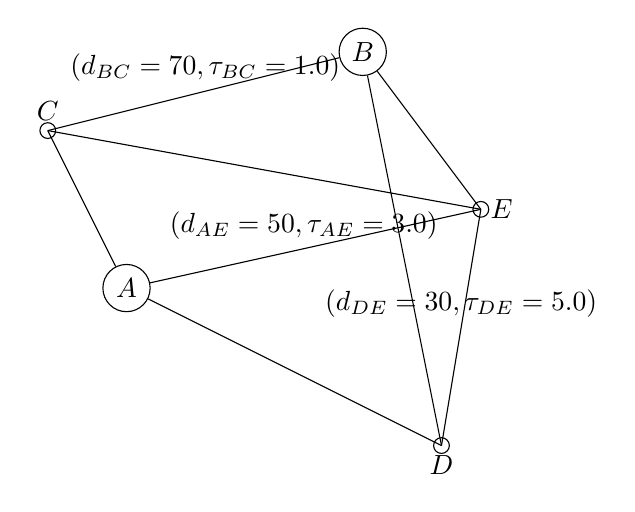
\begin{tikzpicture}
        \draw [] (-1,2) circle [radius=0.1] node [above] at(-1,2) {$C$};
        \draw [] (4,-2) circle [radius=0.1] node [below] at(4,-2) {$D$};
        \draw [] (4.5,1) circle [radius=0.1] node [right] at(4.5,1) {$E$};
        \draw [] (0,0)--(4.5,1) node [above] at(2.25,0.5) {$\left( d_{AE}=50,\tau_{AE}=3.0 \right) $}; 
        \draw [] (4.5,1)--(4,-2) node [above] at(4.25,-0.5) {$\left( d_{DE}=30,\tau_{DE}=5.0 \right) $};
        \draw [] (-1,2)--(4.5,1);
        \draw [] (-1,2)--(3,3) node [above] at(1,2.5) {$(d_{BC}=70,\tau_{BC}=1.0)$};
        \draw [] (4.5,1)--(3,3); 
        \draw [] (4,-2)--(3,3);
        \draw [] (0,0)--(-1,2);
        \draw [] (0,0)--(4,-2);
        \filldraw [color=white] (0,0) circle [radius=0.3];
        \filldraw [color=white] (3,3) circle [radius=0.3];
        \draw [] (0,0) circle [radius=0.3] node at(0,0) {$A$};
        \draw [] (3,3) circle [radius=0.3] node at(3,3) {$B$};
    \end{tikzpicture}
\end{center}
\begin{eg}
    旅行商问题
\end{eg}
\subsection{机器学习}%
\label{sub:机器学习}
\begin{defi}
    学习:

    系统改进其性能的过程(西蒙)

    获取知识的过程(专家系统)

    技能的获取(心理学家)

    事物规律的发现过程
\end{defi}


